\section{Motivation}

Satellite data transmissions have become a key part of critical infrastructure for private, national, and scientific use.
Although new satellites are being launched at a high rate, even decades-old satellites are seeing novel use cases including advanced forest fire detection~\cite{nasaFirms}, analysis of activities in conflict areas~\cite{separatistLuminosity}, emergency communications~\cite{apple_emergency_sos}, and internet service~\textbf{TODO: find citation for e.g. Iridium}.
These systems were built when robust cryptography was uncommon due to less powerful onboard computers.
Additionally, long mission lifespans have lead to a proliferation of satellites that were considered secure at launch, but have since had their master keys leaked or reverse engineered~\cite{lrit-key-dec,xrit-rx}.

It is now well accepted that legacy communications systems without resilient authentication are not robust against modern adversaries.
At the time, this was often not a practical concern since attacks at the physical layer would have required a costly and highly specialized setup.
However, recent decades have seen a significant rise in the off-the-shelf availability of software-defined radio (SDR) hardware which is capable of emitting arbitrary signals at a wide range of frequencies.
This has lowered the barrier to entry for signal injection and denial of service across many wireless systems, including WiFi, wireless sensors, mobile internet~\cite{yang2019hiding,erni2021adaptover}, GNSS~\cite{tippenhauer2011requirements}, and even avionic systems~\cite{sathayeWireless2019}.

Whilst recent news demonstrates that modern adversaries exist and are sufficiently motivated to exploit the downlink~\cite{satcomAnalysis}, the practicality of performing these attacks on satellite downlinks is currently unknown.
This is because achieving signal injection requires that the attacker operates within unique constraints imposed by the physical layer and protocol design of the satellite communications link.

If targeting satellites used for military or high bandwidth communications, this includes transmitting at frequencies higher than the operating range of most SDRs~\cite{esa_satellite_bands}.
Terrestrial attackers against highly directional dish antennas must overcome the attenuation caused by transmitting out of beam, but without saturating the receiver.
The expected polarity of the signal must also be matched.
Additionally, since satellite communications are vulnerable to atmospheric noise, even unencrypted channels are subject to high data integity checks; these must be accounted for when generating the overshadowing signal.

% TODO: is this paragraph necessary considering contributions is coming next?
This work seeks to evaluate the practicality of achieving signal injection attacks in the real world, given these constraints.
We seek to understand how key factors in the design of the satellite affects the required budget and attack complexity.

% TODO: Evaluate downstream consumers?

Several anti-spoofing physical layer countermeasures have been proposed in the academic literature so far, seeking to upgrade the security of existing communications links.
These consider properties such as channel noise, signal timing~\cite{jedermann2021orbit}, signal direction, and fingerprinting the transmitting hardware for continuous probabilistic authentication~\cite{foruhandeh2020spotr,oligeri2020past,borio2016gnss,qiu2022robust}.
However, without a robust threat model for signal injection, no comparative analysis of real world effectiveness of these countermeasures has been possible. % TODO: Outline how the comparative analysis has been limited

\begin{figure}
    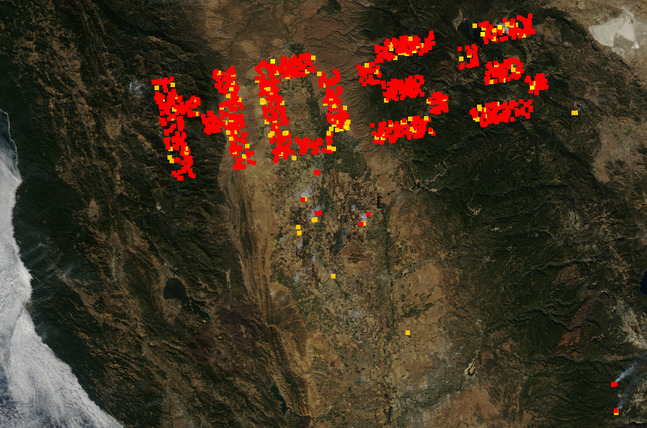
\includegraphics[width=\columnwidth]{diagrams/injection/pixels_800_140.jpg}
    \caption{An injected signal from the attacker manipulates the infrared channels of satellite imagery to create ficticious fires in the resulting dataset.}
    \label{fig:location-injection}
\end{figure}


\subsection{Contributions}

Specifically, we make the following contributions:

\begin{itemize}
    \item We analyze the feasibility of satellite downlink signal injection using commercial off-the-shelf equipment, taking into account the unique constraints of a terrestrial attacker against a highly directional dish;
    \item We show that modern software-defined radios, alongside appropriate mixing and amplifying hardware, is sufficient to inject signals with a low budget;
    \item We demonstrate the effectiveness of this attack type against a representative sample of satellite receiver systems through a full end-to-end case study;
    \item We discuss the impact of similar attacks against other satellite-derived datasets, pointing towards other potentially vulnerable systems, and exploring the effects that an attacker could expect to cause in the real world;
    \item Finally, we examine the applicability of existing countermeasures.
\end{itemize}
